% Apêndices
\begin{apendicesenv}

\partapendices

\chapter{Discussões sobre a verticalização}
\label{appendix:verticalizacao}

Assumindo prédios como paralelepípedos, ou seja, todos os andares apresentam a mesma metragem, é possível traçar relações geométricas nas quais a área ocupada é a superfície que representa a base do paralelepípedo, o número de pavimentos sua altura e a área construída seu volume (Figura \ref{fig:desenho}). Nesse sentido, as relações apresentadas na Equação \ref{eq:pavimentos}, que apresenta diferentes formas de calcular a verticalização, ficam mais claras. Na equação, AC representa a área construída; AO, a área o cupada; AT, a área do terreno; CA o coeficiente de aproveitamento e tx\_ocupacao, o percentual da área do terreno que é ocupada. Usando o procedimento apresentado, em regiões que possuem o mesmo CA, quanto menor for a taxa de ocupação do terreno, maior será a verticalização. Analogamente, para dois lotes com a mesma ocupação de terreno, quanto maior for o CA, maior é a verticalização.

\begin{figure}[h]
    \centering
    \caption{Representação do prédio como um paralelepípedo}
    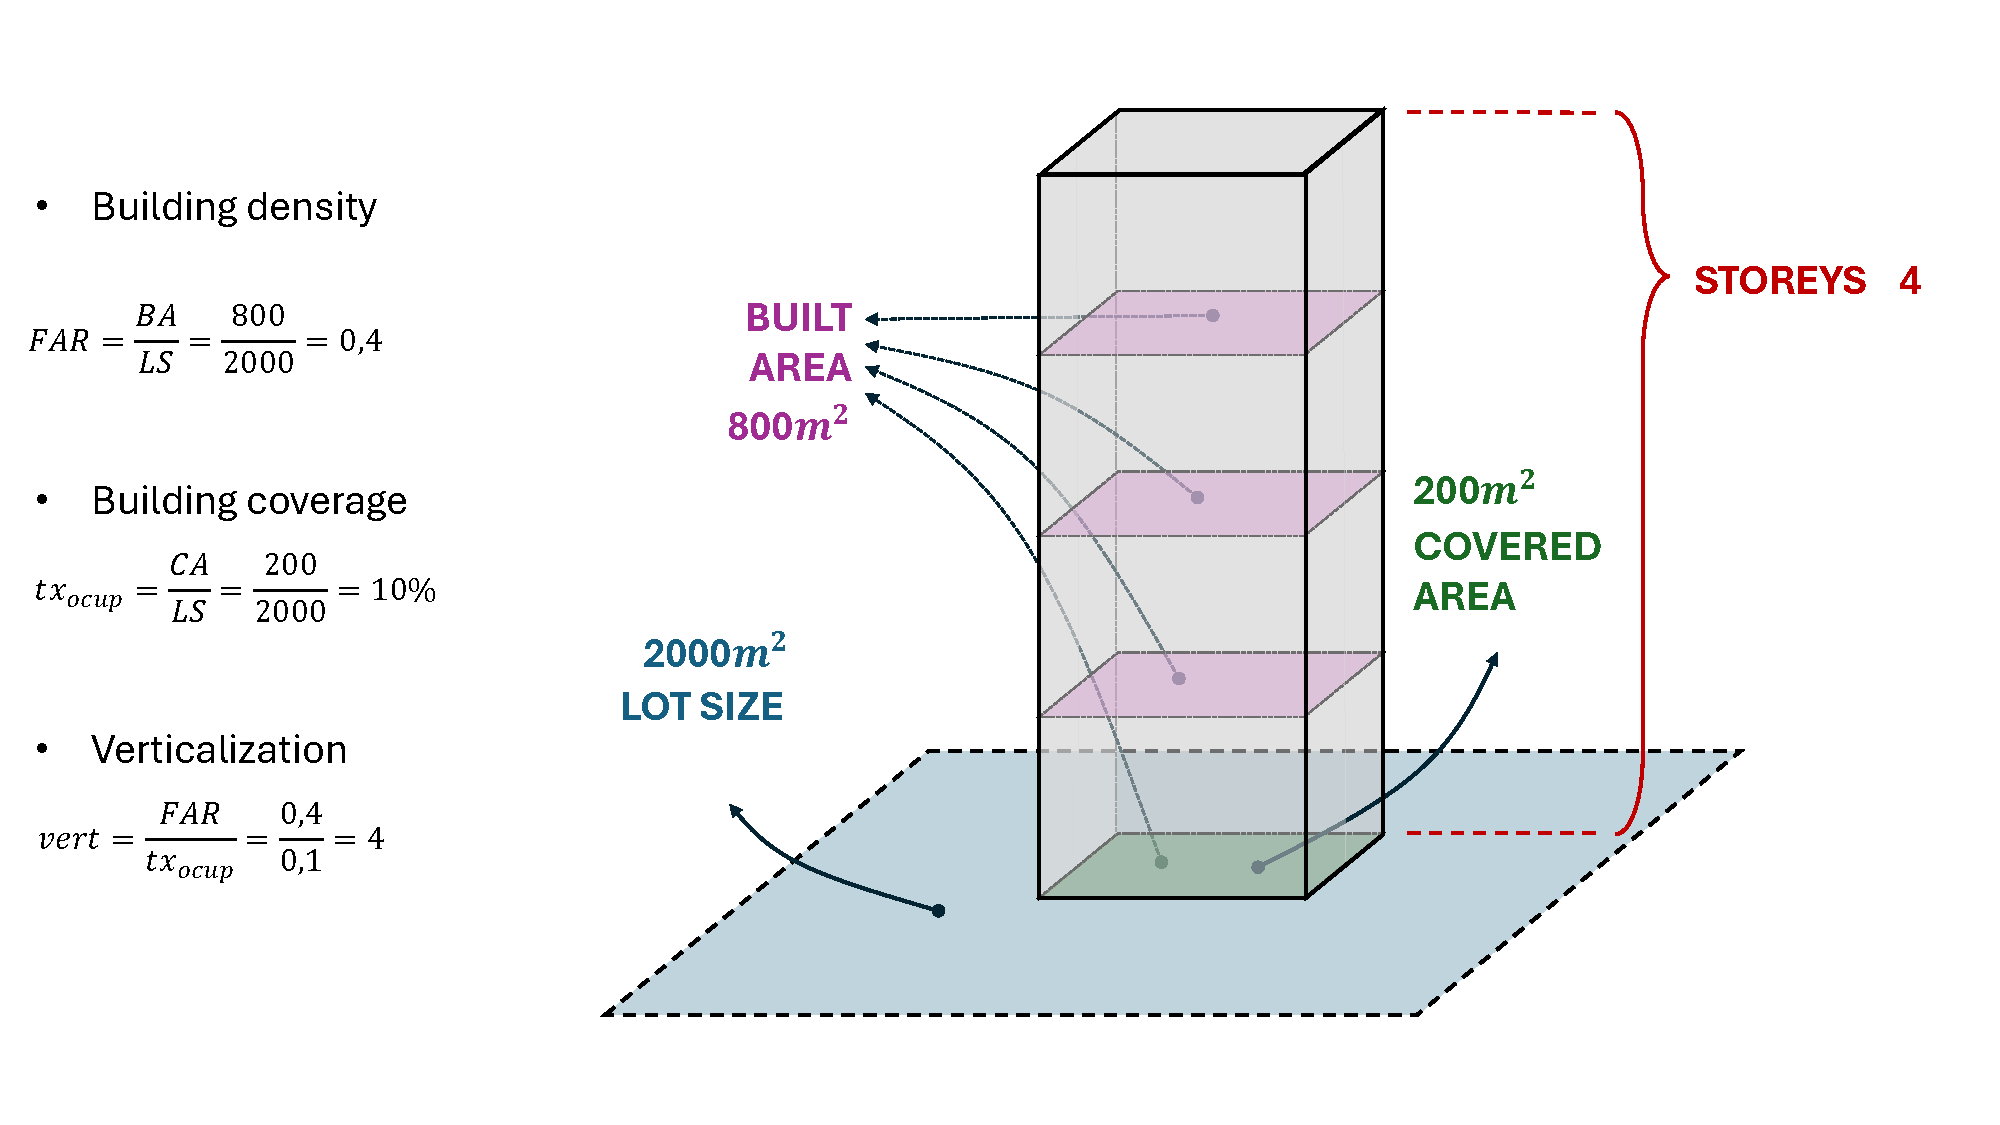
\includegraphics[width = \linewidth]{figuras/desenho.pdf}
    \label{fig:desenho}
\end{figure}

\begin{equation}
    \text{Pavimentos}=\frac{\text{AC}}{\text{AO}}=\frac{\text{AC}}{\text{AT}\cdot\underbrace{\frac{\text{AO}}{\text{AT}}}_\text{tx\_ocup}}=\frac{\text{AC}}{\text{AT}}\div\frac{\text{AO}}{\text{AT}}=\frac{\text{CA}}{\text{tx\_ocup}}
    \label{eq:pavimentos}
\end{equation}
    
Dessa forma, o número de pavimentos nunca será maior do que o CA, dado que a taxa de ocupação sempre é um número que varia entre zero e um. Na Figura \ref{fig:ca-vert} é possível observar a relação entre as duas variáveis nos lotes da cidade de São Paulo. Para lotes muito pequenos, as duas medidas geralmente são iguais, visto que geralmente se ocupa 100\% da área do terreno. Na medida em que a verticalização aumenta, é observável que o CA não acompanha este crescimento, o que indica que há uma queda na taxa de ocupação.

\begin{figure}[h]
    \centering
    \caption{Relação entre densidade construtiva e verticalização nos lotes de São Paulo}
    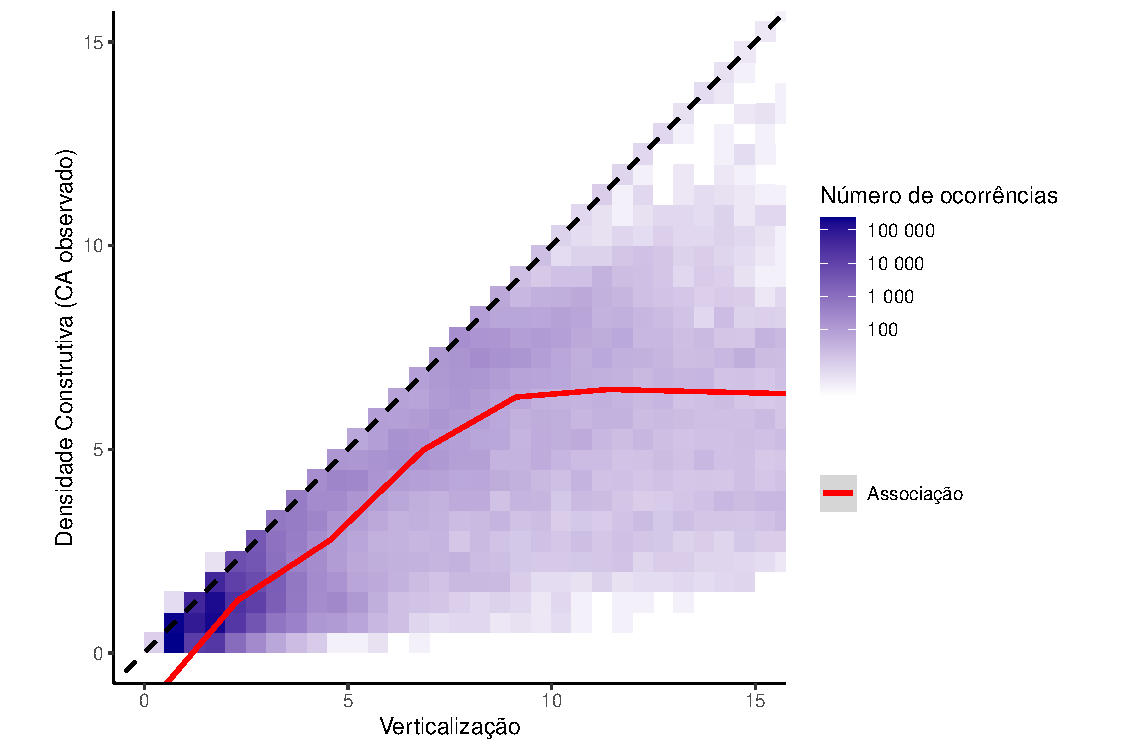
\includegraphics[width = \textwidth]{figuras/ca_vs_verticalizacao.pdf}
    \label{fig:ca-vert}
\end{figure}

\chapter{Metodologia de cruzamento geográfico dos dados}
\label{appendix:cruzamento}

Para combinar dados que estão em níveis de observação geográficos diferentes, é necessário fazer um \textit{join} geográfico. Com isso, é possível identificar todas as geometrias que se interseccionam e escolher um nível para agregá-las. O procedimento decidido nesta pesquisa foi de ponderar pelo percentual da intersecção, dada a necessidade de garantir a precisão dos dados. 

\begin{figure}[h]
    \centering
    \caption{Exemplo de recorte de lote}
    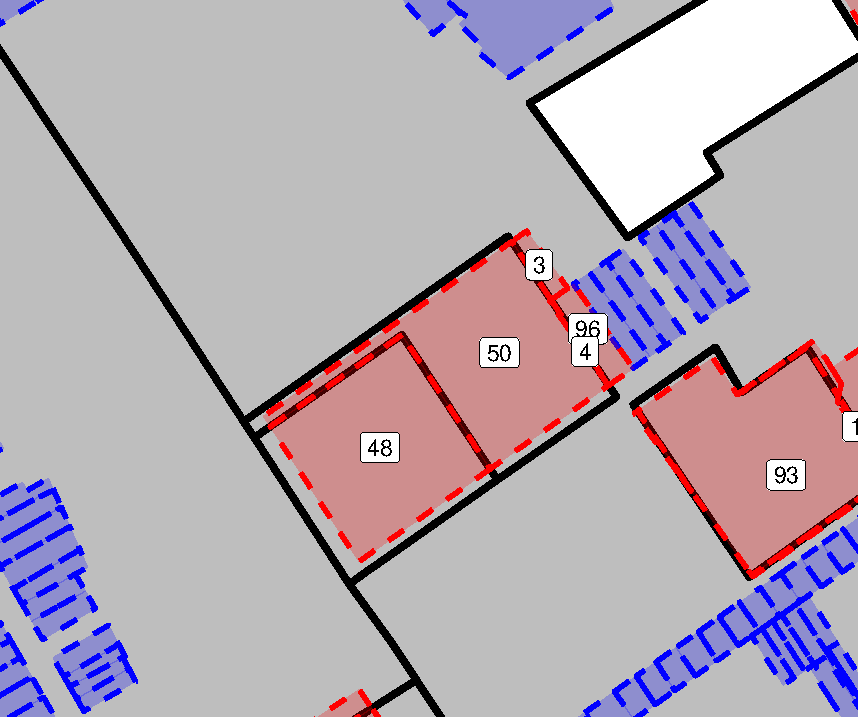
\includegraphics[width = .75\linewidth]{figuras/corte_lote.pdf}
    \label{fig:corte-lote}
\end{figure}

Na Figura \ref{fig:corte-lote} é possível observar um caso da metodologia sendo implementada. No exemplo, estão representados os setores censitários de cinza com contorno preto e os lotes em azul e vermelho com linhas tracejadas. O objetivo neste exemplo é agregar os dados no nível do setor censitário. Dessa forma, quando um lote está presente em mais de um setor censitário, ele é destacado em vermelho é calculada a proporção de sua área que está em cada setor censitário.

A partir disso, é possível distribuir seus atributos de maneira ponderada em cada setor censitário. Se um lote foi dividido no meio, por exemplo, metade das suas unidades habitacionais, área construída, área de lote, etc. são alocadas para um setor, e a outra metade no outro. Este procedimento é impreciso, mas com a granularidade disponível dos dados é o melhor que se pode fazer. Outra abordagem possível seria de calcular o centroide dos lotes e atribuí-los de acordo com qual setor censitário recai, porém o viés neste caso seria maior ainda.

Quando a cidade é recortada em um \textit{raster}, na Seção \ref{sec:perg1}, o mesmo procedimento é realizado, mas é feito o \textit{join} geográfico tanto entre os lotes e o \textit{raster}, quanto entre os setores censitários e o \textit{raster}. Dessa forma, ambos ficam no mesmo nível de observação, garantindo o mínimo de viés possível com os dados disponíveis. O resultado dessa abordagem pode ser observado na Figura \ref{fig:rasters}.

\begin{figure}[h]
    \centering
    \caption{Resultado do cruzamento dos dados a partir do \textit{raster}}
    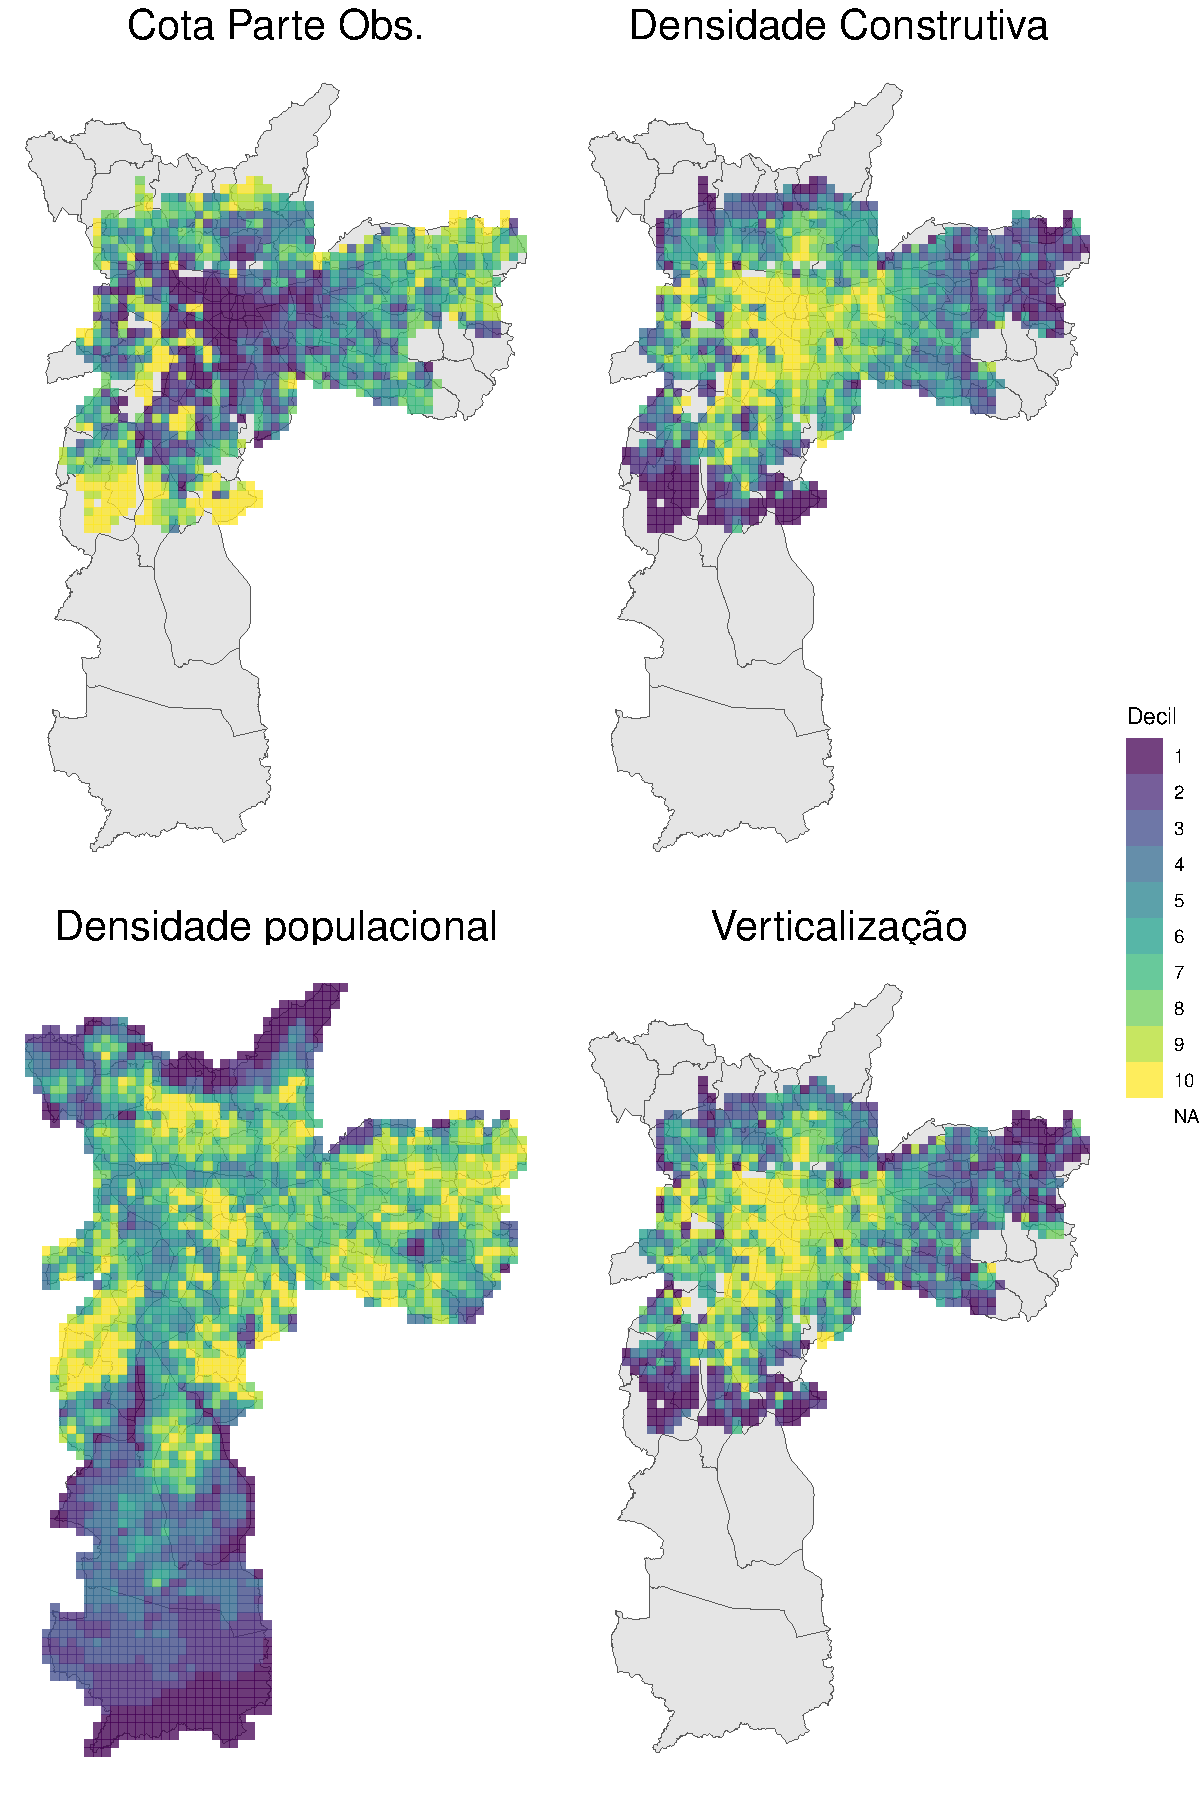
\includegraphics[width = .75\linewidth]{figuras/rasters.pdf}
    \label{fig:rasters}
\end{figure}


\chapter{Discussões sobre a informalidade}
\label{appendix:informalidade}

Para identificar regiões de moradia informal, é essencial comparar as bases de dados para avaliar a coerência das informações. A única variável comparável entre as bases é o número de unidades habitacionais, definido como "unidades" nos dados do IPTU e como "domicílios" no Censo, embora essas categorias possuam definições ligeiramente distintas. A disparidade entre o número de domicílios no Censo e o número de unidades no IPTU pode sugerir a presença de moradias irregulares. Assim, foi criado um "índice de irregularidade", obtido pela razão entre o número de unidades e a soma de unidades e domicílios. Quando esse índice se aproxima de 50\%, as bases são consistentes, indicando que o número de unidades do IPTU é semelhante ao de domicílios no Censo. À medida que o índice se aproxima de 0\%, há uma indicação de que o número de domicílios no Censo é superior ao de unidades no IPTU, apontando para possíveis concentrações de habitações informais.

\begin{itemize}
    \item Definição de domicílios
    
    \begin{quote}
        ``Domicílio é o local estruturalmente separado e independente que se destina a servir de habitação a uma ou mais pessoas, ou que esteja sendo utilizado como tal. A separação fica caracterizada quando o local de habitação for limitado por paredes, muros ou cercas e coberto por um teto, permitindo a uma ou mais pessoas, que nele habitam, isolar-se das demais, com a finalidade de dormir, preparar e/ ou consumir seus alimentos e proteger-se do meio ambiente, arcando, total ou parcialmente, com suas despesas de alimentação ou moradia. A independência fica caracterizada quando o local de habitação tem acesso direto, permitindo a seus moradores entrar e sair sem necessidade de passar por locais de moradia de outras pessoas'' \cite{IBGE2013}.
    \end{quote}

    \item Definição de unidade
    
    No IPTU é considerado que cada contribuinte do IPTU representa uma unidade. Segundo a definição apresentada junto com os dados no portal do GeoSampa, ``A cada imóvel urbano corresponderá um número de inscrição no Cadastro Imobiliário Fiscal, entendendo-se como imóvel: I - a área de terreno, construído ou não, definida em matrícula do competente Serviço de Registro de Imóveis ou em transcrições ainda vigente''
\end{itemize}


Observa-se que os setores censitários periféricos apresentam os maiores índices de irregularidade, conforme evidenciado pelas tonalidades vermelhas na Figura \ref{fig:balanco-raster}, indicando uma discrepância significativa entre as bases do Censo e do IPTU. Tal padrão sugere uma concentração de moradias informais nessas áreas, onde o número de domicílios captado pelo Censo é substancialmente superior ao de unidades cadastradas no IPTU. Esse comportamento não é observado nas áreas centrais da cidade, onde a consistência entre as bases é maior, refletindo uma menor prevalência de habitações informais. Esse índice de irregularidade, portanto, oferece uma ferramenta analítica para identificar espacialmente regiões com potencial presença de loteamentos irregulares e favelas, revelando a distribuição geográfica da informalidade habitacional em São Paulo.

\begin{figure}[h]
    \caption{Padrão geográfico da irregularidade em São Paulo}
    \centering
    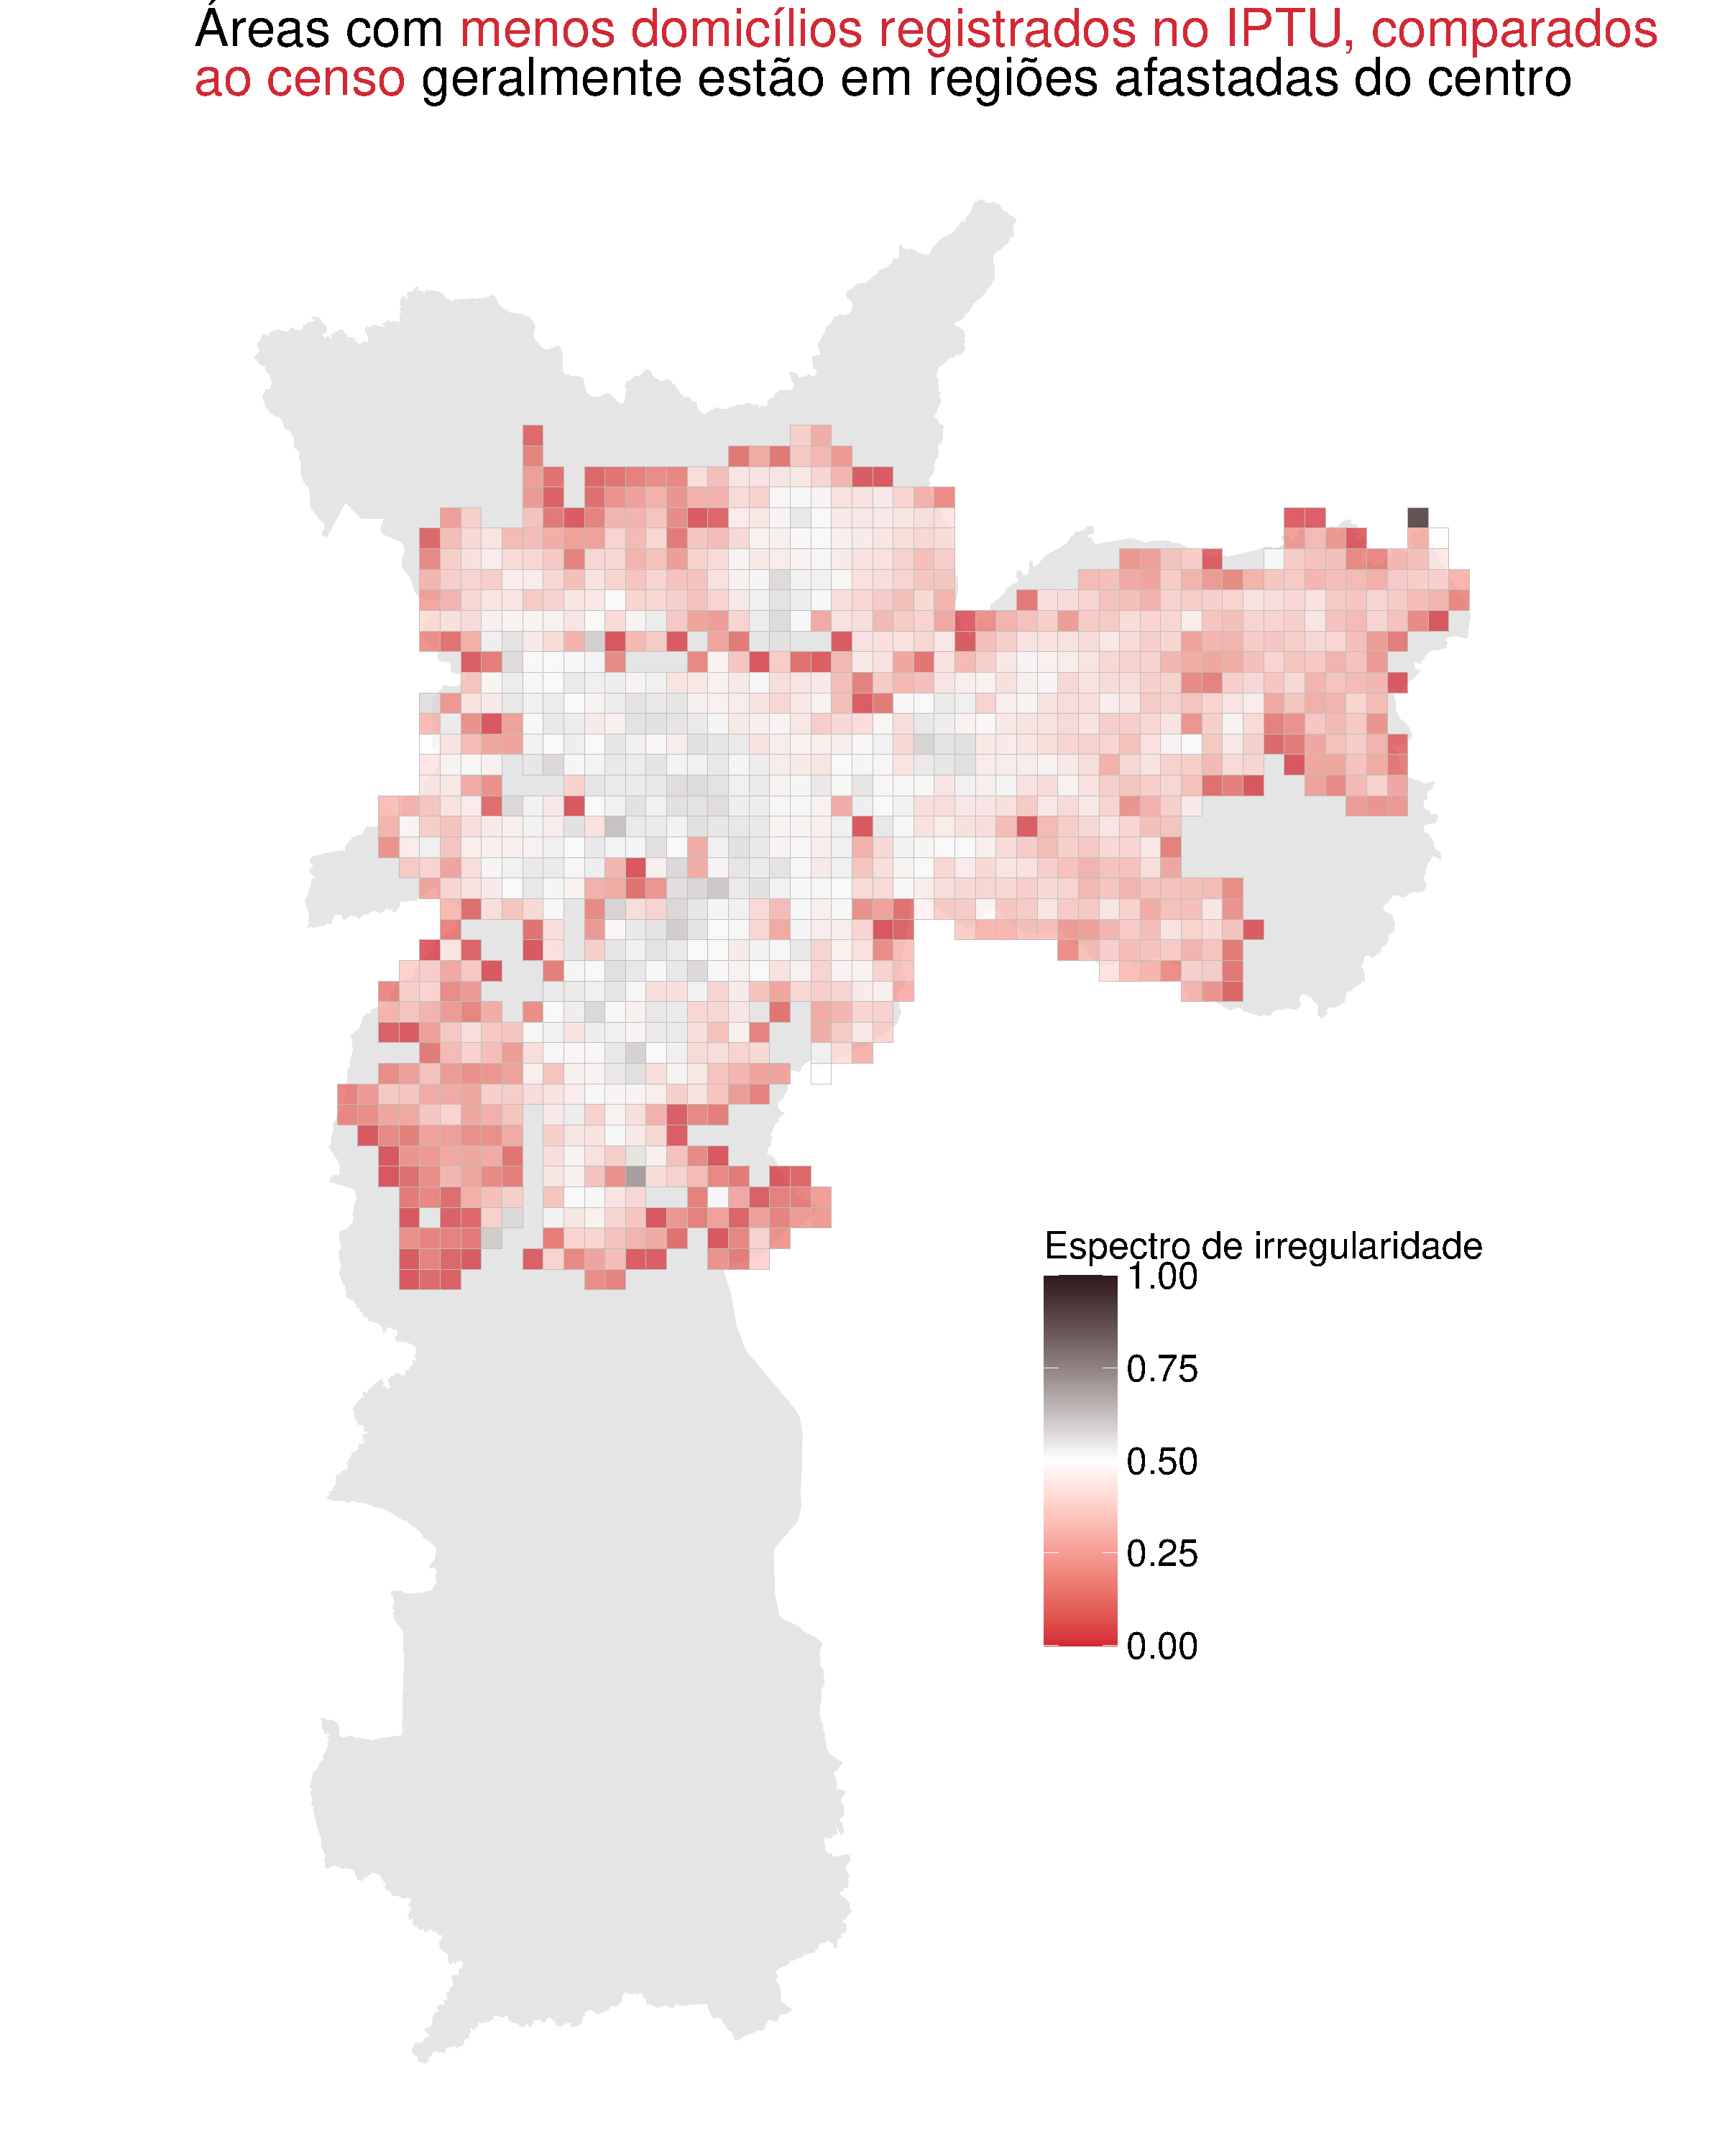
\includegraphics[width = .8\linewidth]{figuras/balanco_raster.pdf}
    \label{fig:balanco-raster}
\end{figure}

\begin{table}[h]
\caption{\textit{raster} cells with the most population density}
\centering
\fontsize{9.8pt}{11.7pt}\selectfont
\begin{tabular*}{.975\linewidth}{@{\extracolsep{\fill}}lrrrrr}
\toprule
 & \multicolumn{4}{c}{Favelas} &  \\ 
\cmidrule(lr){2-5}
Variable & 1. Paraisópolis & 2. Heliópolis  & 4. Paraisópolis & 5. Heliópolis & 3. Sé (Bela Vista) \\ 
\midrule\addlinespace[2.5pt]
Population & 29.598 & 25.280 & 23.824 & 22.920 & 24.576 \\ 
Dwellings (Censo) & 11.655 & 10.178 & 9.361 & 9.001 & 17.875 \\ 
Dwellings Occupied & 10.791 & 9.269 & 8.810 & 8.274 & 13.732 \\ 
Dwellings (IPTU) & 0 & 1.857 & 7 & 3 & 21.057 \\ 
Irregularity Spectrum & 0.00\% & 15.43\% & 0.08\% & 0.03\% & 54.09\% \\ 
Population Density & 46.247 & 39.500 & 37.225 & 35.813 & 38.400 \\ 
Area & 640.000 & 640.000 & 640.000 & 640.000 & 640.000 \\ 
\bottomrule
\label{tab:top5}

\end{tabular*}
\end{table}



Na Tabela \ref{tab:top5} estão descritas as 5 células do \textit{raster} que apresentam maior densidade populacional. É interessante observar que 4 das 5 células mais densas da cidade são de territórios de favelas e repletos quase completamente de domicílios que não estão registrados no IPTU. A densidade populacional do município de São Paulo no geral é de 7.529 habitantes por quilômetro quadrado, o que significa que esta célula do \textit{raster} posicionada na região de Paraisópolis apresenta uma densidade quase quatro vezes maior do que o resto da cidade. Outro fator interessante é o número maior de unidades no IPTU na região da Sé, se comparadas com domicílios do censo. Esta é uma das poucas regiões em que o espectro de irregularidade ultrapassa 50\%. Isso pode estar associada a alta taxa de abandono, que dificulta a medição por parte dos entrevistadores -- os dados do Censo indicam que 34,8\% dos domicílios desta célula do \textit{raster} estão desocupados.

\chapter{Verticalização e adensamento nos bairros paulistanos}
\label{appendix:bairros}

\begin{figure}[!h]
    \centering
    \caption{Densidade populacional de padrões construtivos nos bairros paulistanos}
    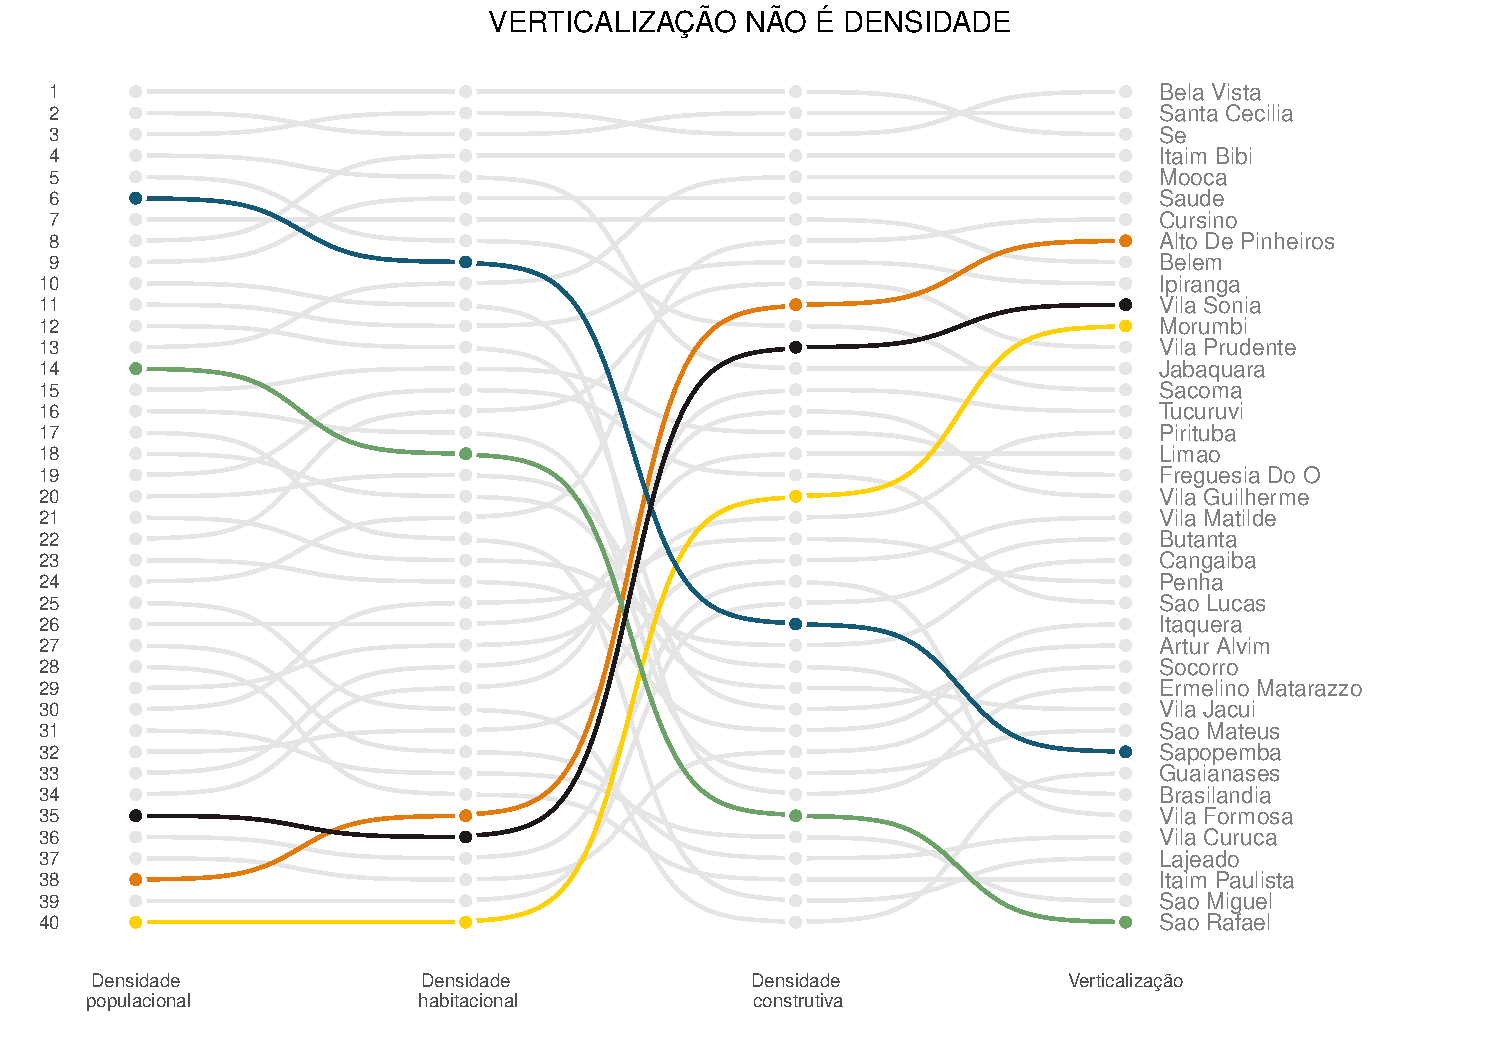
\includegraphics[width = \linewidth]{figuras/bairros.pdf}
    \label{fig:bairros}
\end{figure}


As análises nas Figuras \ref{fig:bairros} e \ref{fig:bairros-mapa} destacam as disparidades entre verticalização e densidade populacional nos bairros de São Paulo. No primeiro caso, bairros como Jardim Paulista, Moema e Pinheiros exemplificam regiões altamente verticalizadas que, paradoxalmente, não apresentam elevada densidade populacional. Por outro lado, bairros periféricos como Capão Redondo possuem alta densidade populacional, mas baixa verticalização, refletindo um padrão de ocupação horizontal e adensamento intenso. Na Figura \ref{fig:bairros}, foram selecionados 40 entre os 96 distritos que apresentam o espectro de irregularidade mais próximo de 50\%, ou seja, os dados do Censo e do IPTU são parecidos. O especial destes bairros é que os dados do IPTU são mais confiáveis.

Na Figura \ref{fig:bairros-mapa}, é possível visualizar em um mapa onde estão os bairros em que a diferença entre a posição no ranqueamento da densidade populacional e da verticalização é maior. Nos bairros vermelhos, nos quais esta distância é muito grande, há presença de verticalização sem adensamento. Na Figura \ref{fig:bairros-mapa-CP}, o mesmo mapa é criado, mas para verificar em quais regiões não se observa que a cota parte é traduzida em densidade populacional. Como a densidade populacional é o fator mais importante para definir a densidade populacional, são raros os casos em que a posição no ranqueamento diverge, e quando acontece, são poucas posições. Ainda assim, nos bairros pintados de vermelhos menos pessoas habitam cada residência, o que pode estar associado à forte presença de apartamentos estúdio, enquanto os azuis apontam para regiões nas quais as residências são ocupadas por núcleos familiares maiores. 

\begin{figure}[!h]
    \centering
    \caption{Diferença entre posição da densidade populacional e verticalização no ranqueamento dos bairros}
    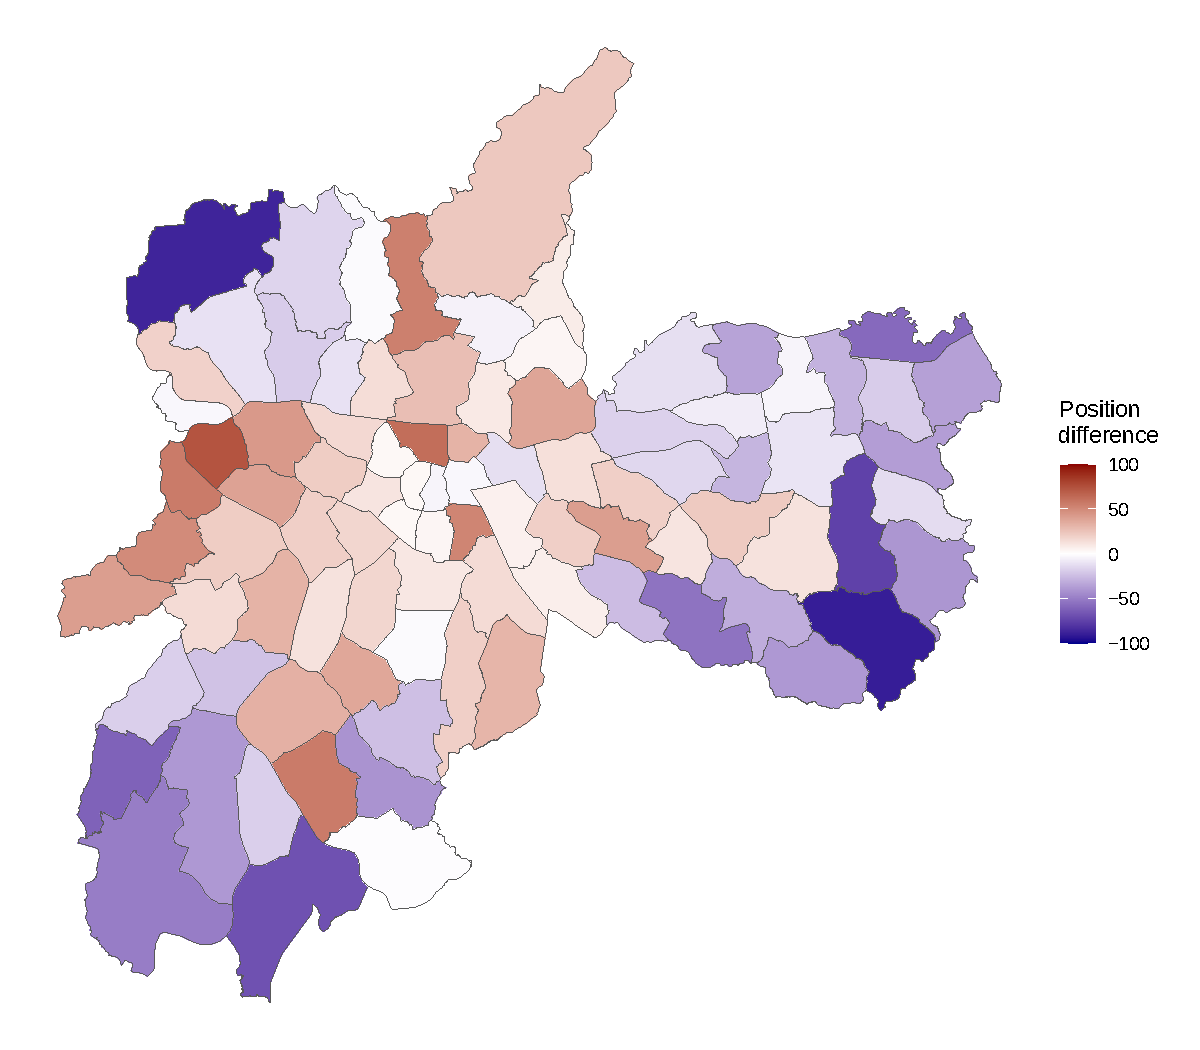
\includegraphics[width = \linewidth]{figuras/bairros-mapa.pdf}
    \label{fig:bairros-mapa}
\end{figure}

\begin{figure}[!h]
    \centering
    \caption{Diferença entre posição da densidade populacional e densidade habitacional no ranqueamento dos bairros}
    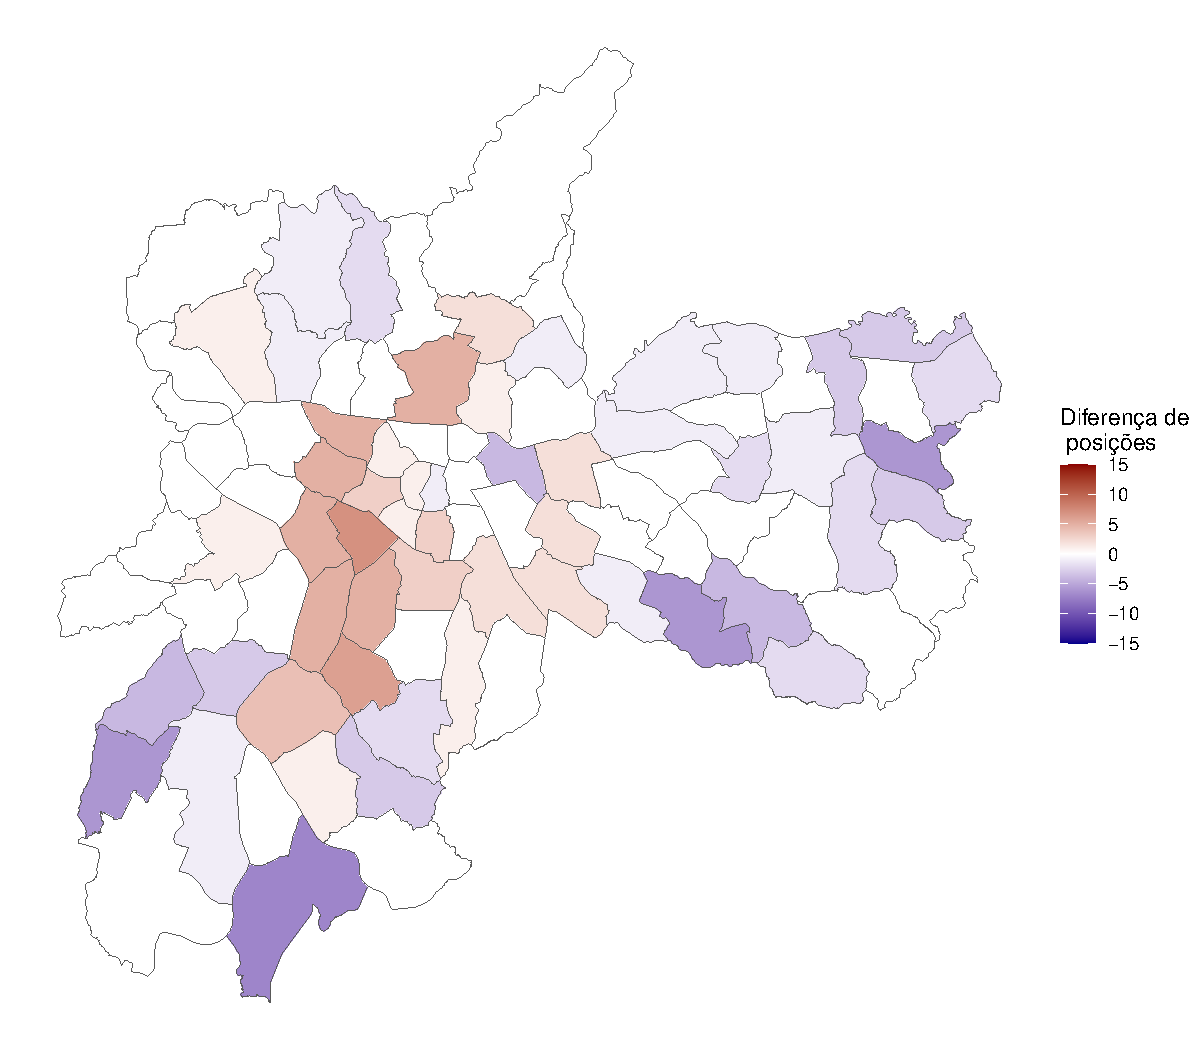
\includegraphics[width = \linewidth]{figuras/bairros-mapa-cotaparte.pdf}
    \label{fig:bairros-mapa-CP}
\end{figure}





\chapter{Robustez dos resultados}
\label{appendix:robustez}

\begin{figure}[!h]
    \centering
    \caption{Robustez dos resultados da regressão para diferentes espectros de irregularidade}
    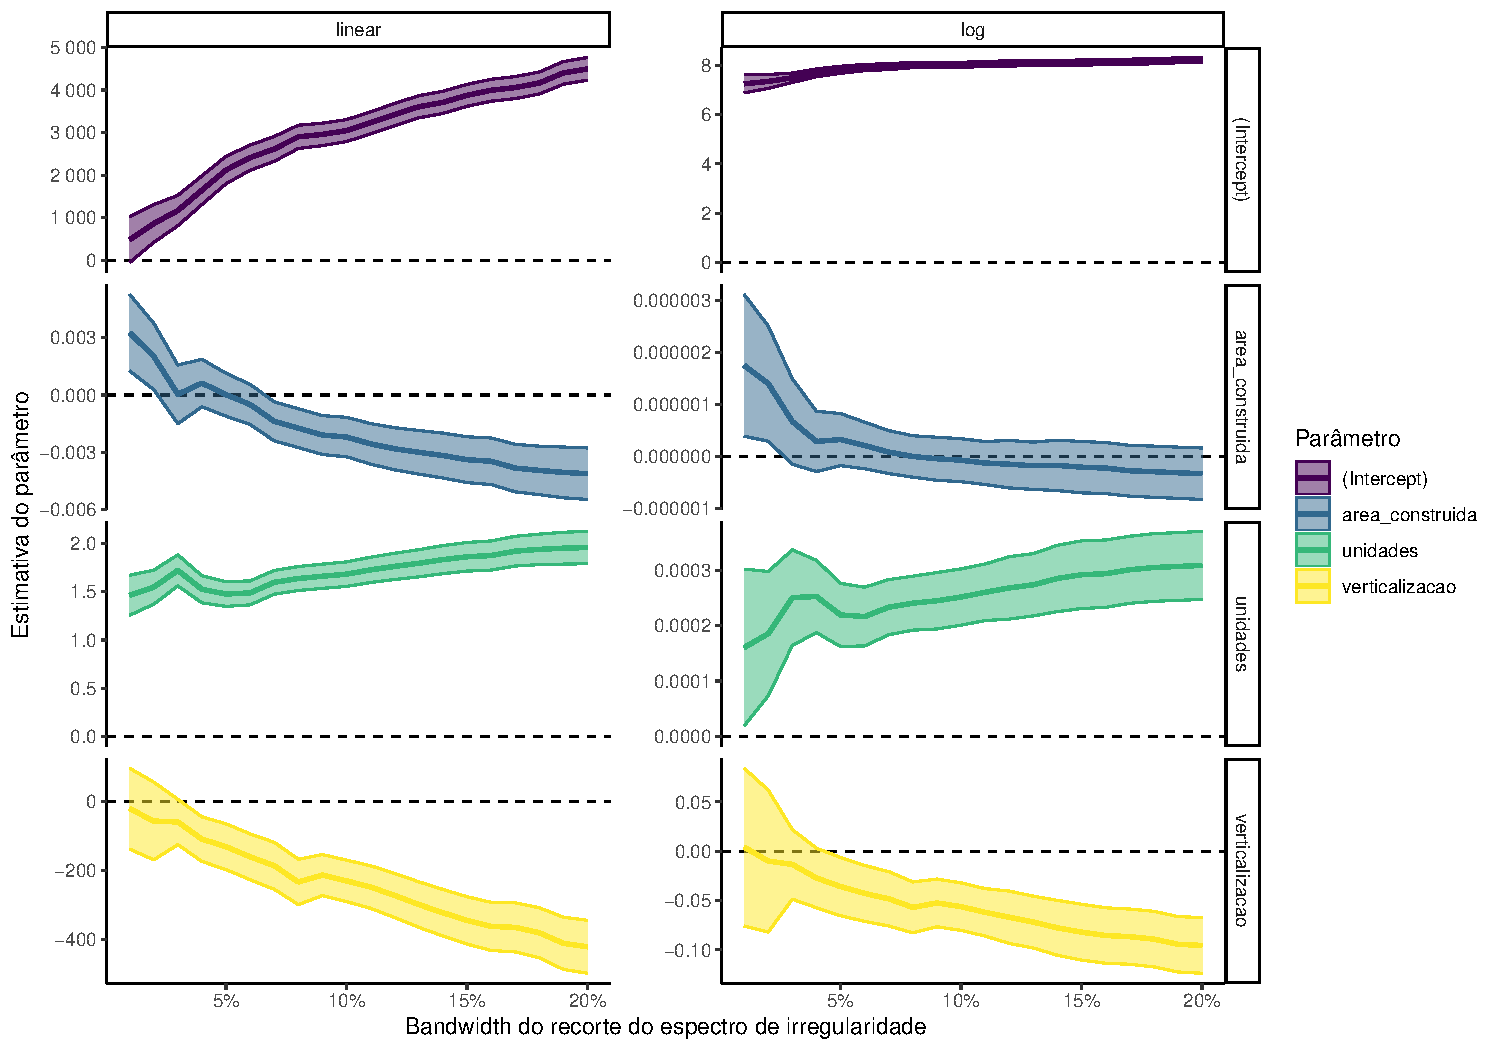
\includegraphics[width = \linewidth]{figuras/robustez-regressao1pop.pdf}
    \label{fig:robustez-reg1}
\end{figure}


\begin{figure}[!h]
    \centering
    \caption{Robustez dos resultados do DiD para diferentes recortes de proximidade na análise do IPTU}
    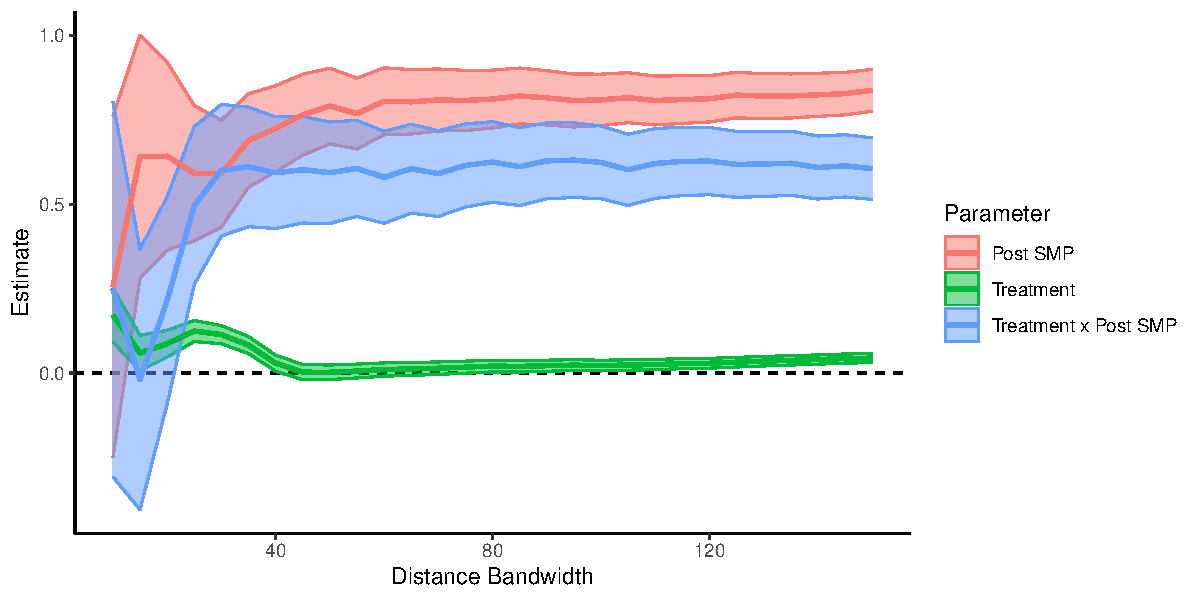
\includegraphics[width = \linewidth]{figuras/did-IPTU-bandas.pdf}
    \label{fig:robustez-did-IPTU}
\end{figure}

\begin{figure}[!h]
    \centering
    \caption{Robustez dos resultados do DiD para diferentes recortes de proximidade na análise do Censo. (Tabela \ref{tab:did-censo}, coluna B e D)}
    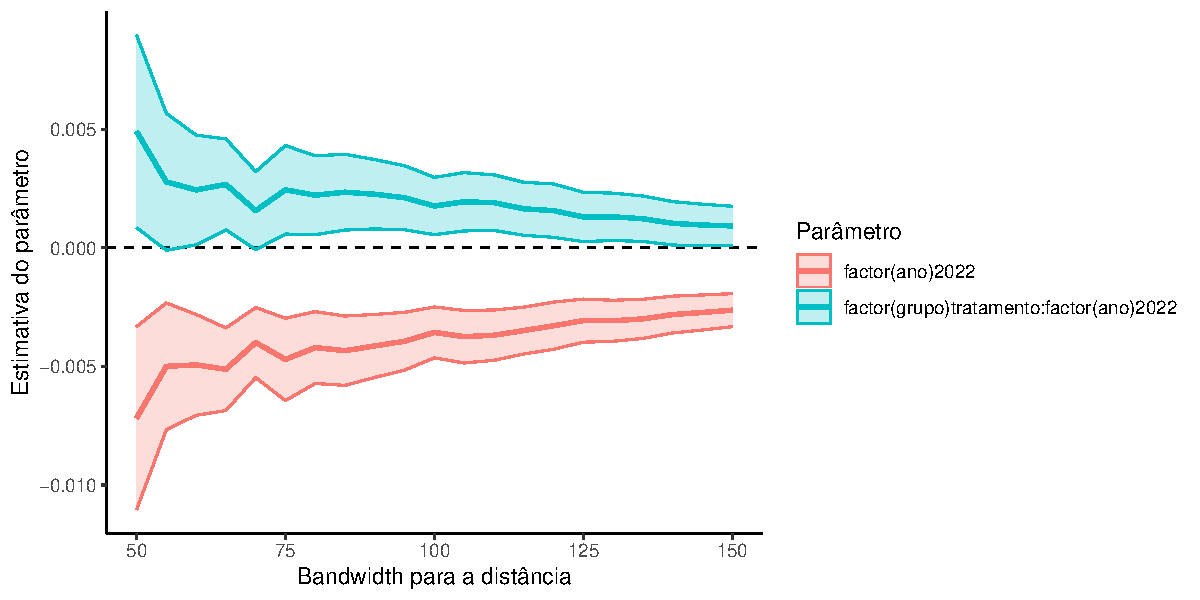
\includegraphics[width = \linewidth]{figuras/did-censo-bandas.pdf}
    \label{fig:robustez-did-censo}
\end{figure}















\chapter{Outras figuras e tabelas}
\label{appendix:figuras}

\clearpage

\begin{figure}[h]
    \centering
    \caption{Variação no tempo dos padrões construtivos residenciais observados em São Paulo}
    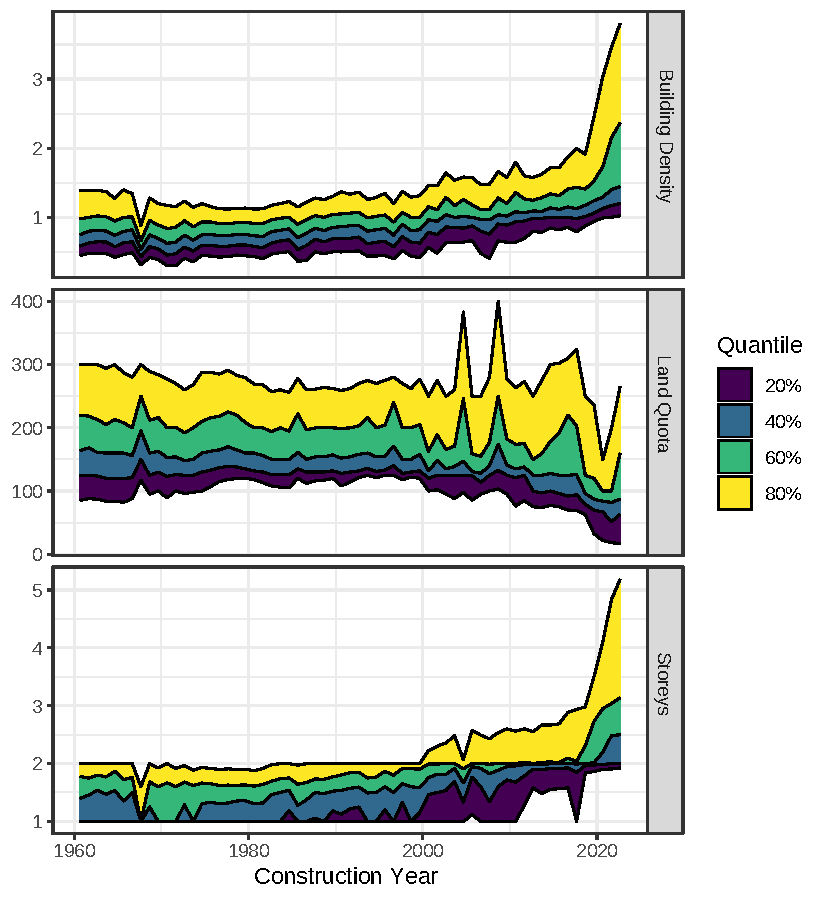
\includegraphics[width = .75\linewidth]{figuras/indicadores_tempo.pdf}
    \label{fig:indicadores-tempo}
\end{figure}

Ao analisar os padrões construtivos ao longo do tempo na Figura \ref{fig:indicadores-tempo}, fica evidente a trajetória de adensamento. Na figura, cada linha representa um quantil dos lotes do IPTU. Ao ordenar as construções no ano 2020 de maneira crescente de CA observado, o empreendimento na posição 80\% dessa fila apresenta um CA observado de 3,8. Este mesmo procedimento nos anos 2000 retornaria um empreendimento com CA observado igual a 1,46. Analogamente, a cota parte observada que em 2020 apresenta o quantil 20\% de meros 21,7 metros quadrados, no ano 2000 apresentaria 100 metros quadrados. Isso evidencia que nos últimos anos São Paulo passou por um forte processo de adensamento.


\clearpage

\begin{figure}
    \centering
    \caption{Área construída no município de São Paulo por tipo e padrão de uso}
    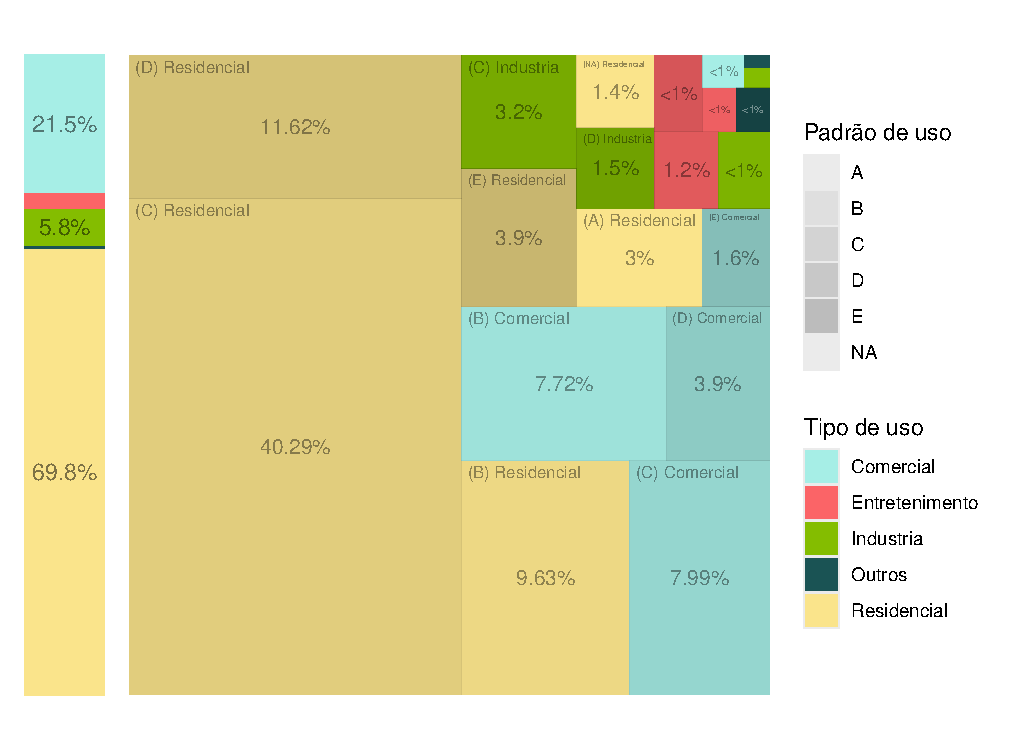
\includegraphics[width = .8\linewidth]{figuras/tree_area_construida.pdf}
    \label{fig:area_construida}
\end{figure}

Na Figura \ref{fig:area_construida}, é possível observar a distribuição da área construída por tipo e padrão de uso. Em São Paulo, 70\% da área construída é residencial, sendo que o padrão residencial mais comum é o "C". O padrão é uma divisão feita no cálculo do IPTU \cite{lei10235_1986}, para criar descontos do imposto para imóveis com características desejáveis do ponto de vista do planejamento urbano, como maior adensamento, ou para imóveis de pessoas com menor poder aquisitivo. Medidas como metragem, pé direito, vaga de garagem, número de pavimentos, elementos arquitetônicos, materiais de construção, etc., são fatores levados em consideração para determinar o padrão. No caso do "C", ele está no meio da escala de densidade, sendo "A" o mais denso, e "E" o menos. O segundo uso mais comum é o comercial, seguido do industrial e entretenimento. Na categoria de entretenimento, se encontram templos religiosos, clubes, estádios esportivos, cinemas, aeroporto, museu, zoológico, entre outros.






\begin{figure}[!h]
    \centering
    \caption{Regiões de eixos (pintadas em azul)}
    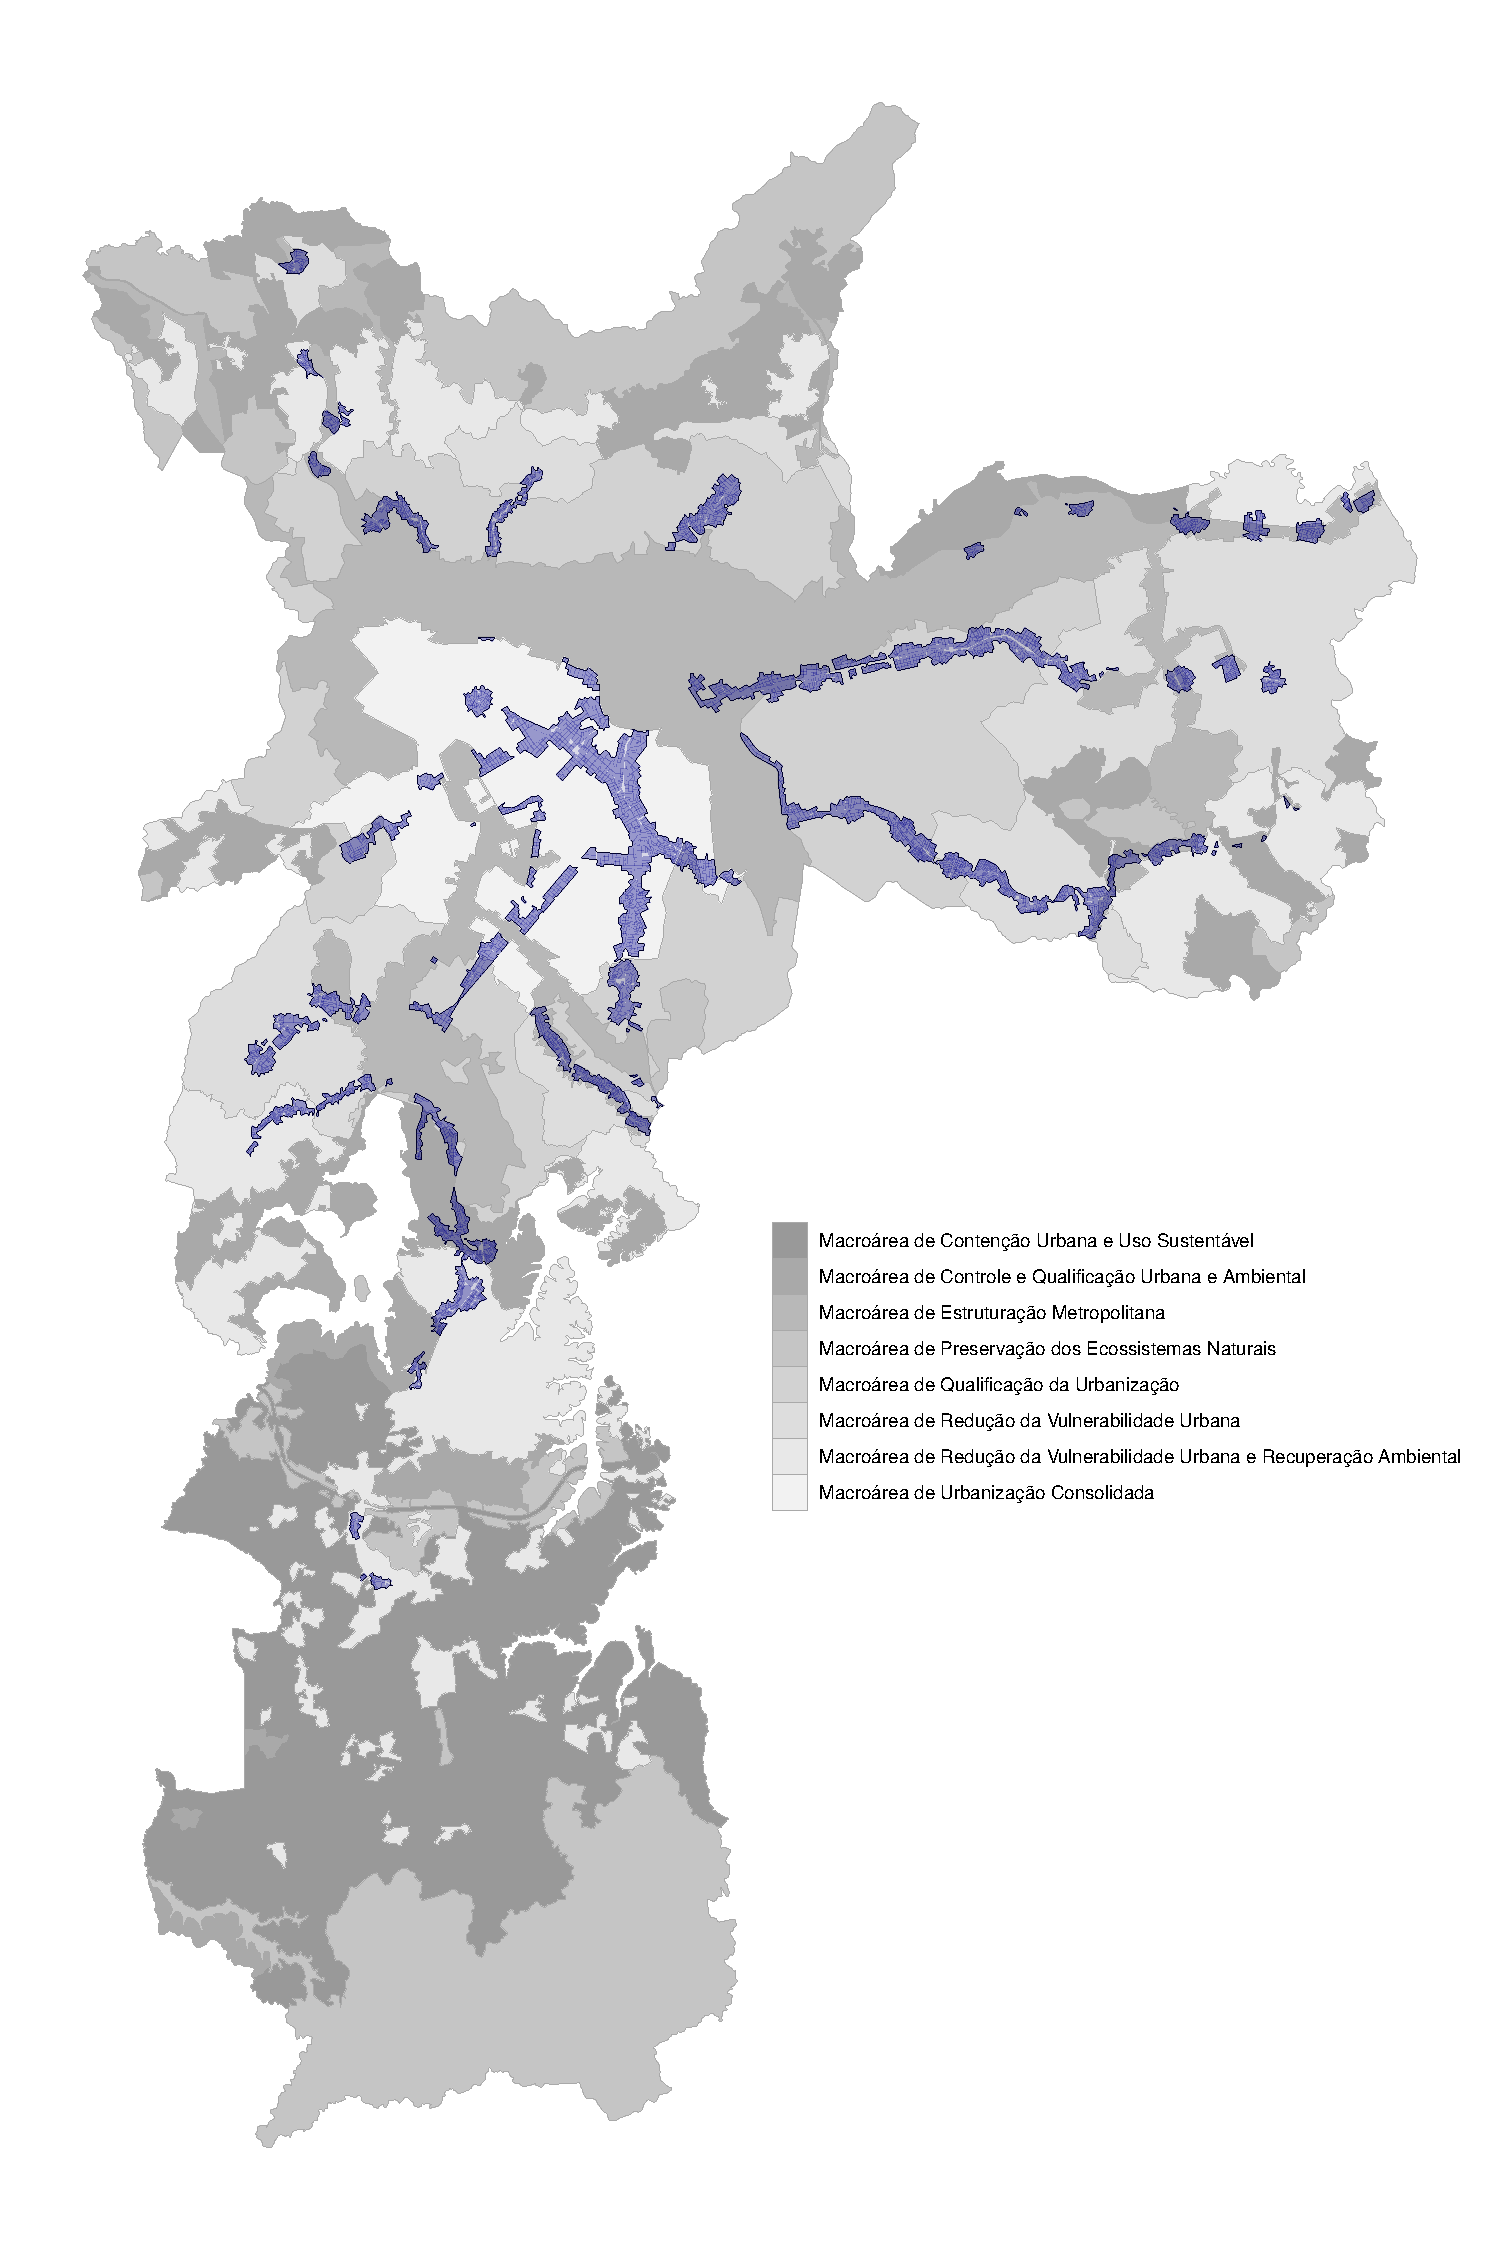
\includegraphics[width = .85\linewidth]{figuras/macroareas-eixos.pdf}
    \label{fig:eixos}
\end{figure}

\clearpage

\begin{figure}[!h]
    \centering
    \caption{Distribuição da quantidade de moradores em cada célula do raster}
    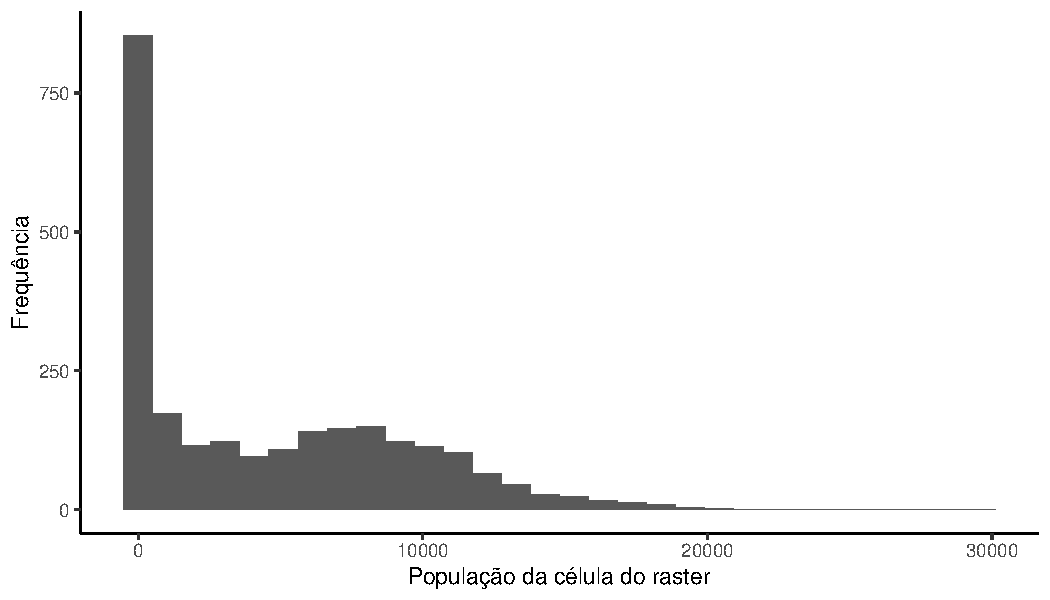
\includegraphics[width = .85\linewidth]{figuras/populacao-distribuicao-raster.pdf}
    \label{fig:populacao-rasters}
\end{figure}






\end{apendicesenv}
    
    